% !TEX root = ../main.tex
\section{Experiments}
We experiment on two few-shot classification datasets, \textit{mini}-ImageNet and
\textit{tiered}-ImageNet. Both are subsets of ImageNet~\citep{imagenet}, with images sizes reduced
to $84 \times 84$ pixels. We also modified the datasets to accommodate the
incremental few-shot learning settings.
\footnote{Code released at: \url{https://github.com/renmengye/inc-few-shot-attractor-public}}
\subsection{Datasets}
\iflatexml
\begin{itemize}
\item \textbf{\textit{mini}-ImageNet}
Proposed by \citet{matching}, \textit{mini}-ImageNet
contains 100 object classes and 60,000 images. We used the splits proposed by \citet{metalstm}, where
training, validation, and testing have 64, 16 and 20 classes respectively.
\item \textbf{\textit{tiered}-ImageNet}
Proposed by \citet{fewshotssl}, \textit{tiered}-ImageNet is a
larger subset of ILSVRC-12. It features a categorical split among training, validation, and testing
subsets. The categorical split means that classes that belong to the same high-level category, e.g.
“working dog” and "terrier" or some other dog breed, are not split between training, validation and
test. This is a harder task, but one that more strictly evaluates generalization to new classes. It
is also  an order of magnitude larger than \textit{mini}-ImageNet.
\end{itemize}
\else
\begin{itemize}[leftmargin=*]
\item \textbf{\textit{mini}-ImageNet}
Proposed by \citet{matching}, \textit{mini}-ImageNet
contains 100 object classes and 60,000 images. We used the splits proposed by \citet{metalstm}, where
training, validation, and testing have 64, 16 and 20 classes respectively.
\item \textbf{\textit{tiered}-ImageNet}
Proposed by \citet{fewshotssl}, \textit{tiered}-ImageNet is a
larger subset of ILSVRC-12. It features a categorical split among training, validation, and testing
subsets. The categorical split means that classes that belong to the same high-level category, e.g.
“working dog” and "terrier" or some other dog breed, are not split between training, validation and
test. This is a harder task, but one that more strictly evaluates generalization to new classes. It
is also  an order of magnitude larger than \textit{mini}-ImageNet.
\end{itemize}
\fi

% !TEX root = ../main.tex
\begin{table}
\centering
\caption{Comparison of our proposed model with other methods}
\renewcommand{\arraystretch}{1.2}
\label{}
\begin{small}
% \begin{tabular}{l|p{2.8cm}|p{2.5cm}|p{2.8cm}}
\begin{tabular}{lp{3.2cm}p{2.5cm}p{3.8cm}}
\toprule
Method           & Few-shot learner     & Episodic objective      & Attention mechanism \\
% \hline\hline
\midrule
Imprint 
\citep{qi2018imprinting}         
                 & Prototypes          & N/A                     & N/A                \\
\hline
LwoF \citep{lwof} & Prototypes + base classes & N/A         & Attention on base classes      \\
\hline
Ours             & A fully trained classifier & Cross entropy on novel classes & Attention on learned attractors \\
\bottomrule
\end{tabular}
\end{small}
\end{table}
% !TEX root = ../main.tex
\iflatexml
\begin{table}[t]
\vspace{-0.3in}
\begin{minipage}[t]{0.49\textwidth}
\begin{small}
\begin{center}
\caption{\textit{mini}-ImageNet 64+5-way results}
\vspace{-0.1in}
\label{tab:fewshot1}
\resizebox{\columnwidth}{!}{
\begin{tabular}{c|cc|cc}
\toprule
\multirow{2}{*}{Model} & \multicolumn{2}{c|}{1-shot}           & \multicolumn{2}{c}{5-shot} \\
          & Acc. $\uparrow$ & $\Delta \downarrow$ & Acc. $\uparrow$ & $\Delta \downarrow$ \\
\midrule
ProtoNet  & 42.73 $\pm$ 0.15      & -20.21      & 57.05 $\pm$ 0.10      & -31.72      \\
Imprint   & 41.10 $\pm$ 0.20      & -22.49      & 44.68 $\pm$ 0.23      & -27.68      \\
LwoF      & 52.37 $\pm$ 0.20      & -13.65      & 59.90 $\pm$ 0.20      & -14.18      \\
Ours      & \tb{54.95} $\pm$ 0.30 & -11.84      & \tb{63.04} $\pm$ 0.30 & \tb{-10.66} \\
\bottomrule
\end{tabular}
}
\end{center}
\end{small}
\end{minipage}
\hfill
\begin{minipage}[t]{0.49\textwidth}
\begin{small}
\begin{center}
\caption{\textit{tiered}-ImageNet 200+5-way results}
\vspace{-0.1in}
\label{tab:fewshot2}
% \resizebox{\columnwidth}{!}{
\begin{tabular}{c|cc|cc}
% \hline
\toprule
\multirow{2}{*}{Model} & \multicolumn{2}{c|}{1-shot} & \multicolumn{2}{c}{5-shot}  \\
 & Acc. $\uparrow$ & $\Delta \downarrow$ & Acc. $\uparrow$ & $\Delta \downarrow$    \\
% \hline\hline
\midrule
ProtoNet  & 30.04 $\pm$ 0.21 & -29.54 & 41.38 $\pm$ 0.28 & -26.39      \\
Imprint   & 39.13 $\pm$ 0.15 & -22.26 & 53.60 $\pm$ 0.18 & -16.35 \\
LwoF      & 52.40 $\pm$ 0.33 & -8.27  & 62.63 $\pm$ 0.31 & -6.72            \\
Ours      &  \tb{56.11} $\pm$ 0.33 & \tb{-6.11}  & \tb{65.52} $\pm$ 0.31 & \textbf{-4.48} \\
\bottomrule
\end{tabular}
% }
\end{center}
\end{small}
\end{minipage}
% \begin{center}
{$\Delta=$ average decrease in acc. caused by  \emph{joint} prediction within base and novel classes ($\Delta = \frac{1}{2} (\Delta_a+\Delta_b)$)\\
$\uparrow\, (\downarrow)$ represents higher (lower) is better.}
% \end{center}
\vspace{-0.2in}
\end{table}
\else
\begin{table}[t]
\vspace{-0.3in}
\begin{minipage}[t]{0.49\textwidth}
\begin{small}
\begin{center}
\caption{\textit{mini}-ImageNet 64+5-way results}
\vspace{-0.1in}
\label{tab:fewshot1}
\resizebox{\columnwidth}{!}{
\begin{tabular}{c|cc|cc}
\toprule
\multirow{2}{*}{Model} & \multicolumn{2}{c|}{1-shot}           & \multicolumn{2}{c}{5-shot} \\
          & Acc. $\uparrow$ & $\Delta \downarrow$ & Acc. $\uparrow$ & $\Delta \downarrow$ \\
\midrule
ProtoNet \citep{proto}
          & 42.73 $\pm$ 0.15      & -20.21      & 57.05 $\pm$ 0.10      & -31.72      \\
Imprint \citep{qi2018imprinting}
          & 41.10 $\pm$ 0.20      & -22.49      & 44.68 $\pm$ 0.23      & -27.68      \\
LwoF \citep{lwof}
          & 52.37 $\pm$ 0.20      & -13.65      & 59.90 $\pm$ 0.20      & -14.18      \\
Ours      & \tb{54.95} $\pm$ 0.30 & -11.84      & \tb{63.04} $\pm$ 0.30 & \tb{-10.66} \\
\bottomrule
\end{tabular}
}
\end{center}
\end{small}
\end{minipage}
\hfill
\begin{minipage}[t]{0.49\textwidth}
\begin{small}
\begin{center}
\caption{\textit{tiered}-ImageNet 200+5-way results}
\vspace{-0.1in}
\label{tab:fewshot2}
\resizebox{\columnwidth}{!}{
\begin{tabular}{c|cc|cc}
% \hline
\toprule
\multirow{2}{*}{Model} & \multicolumn{2}{c|}{1-shot} & \multicolumn{2}{c}{5-shot}  \\
 & Acc. $\uparrow$ & $\Delta \downarrow$ & Acc. $\uparrow$ & $\Delta \downarrow$    \\
% \hline\hline
\midrule
ProtoNet \citep{proto} & 30.04 $\pm$ 0.21 & -29.54 & 41.38 $\pm$ 0.28 & -26.39      \\
Imprint \citep{qi2018imprinting}
& 39.13 $\pm$ 0.15 & -22.26 & 53.60 $\pm$ 0.18 & -16.35 \\
LwoF \citep{lwof} & 52.40 $\pm$ 0.33 & -8.27  & 62.63 $\pm$ 0.31 & -6.72            \\
Ours        &  \tb{56.11} $\pm$ 0.33 & \tb{-6.11}  & \tb{65.52} $\pm$ 0.31 & \textbf{-4.48} \\
\bottomrule
\end{tabular}
}
\end{center}
\end{small}
\end{minipage}
\begin{center}
{\footnotesize $\Delta=$ average decrease in acc. caused by  \emph{joint} prediction within base and novel classes ($\Delta = \frac{1}{2} (\Delta_a+\Delta_b)$)\\
$\uparrow\, (\downarrow)$ represents higher (lower) is better.}
\end{center}
\vspace{-0.2in}
\end{table}
\fi

\subsection{Experiment setup}
We use a standard ResNet backbone~\citep{resnet} to learn the feature representation through
supervised training. For \textit{mini}-ImageNet experiments, we follow \citet{mishra2017meta} and use
a modified version of ResNet-10. For \textit{tiered}-ImageNet, we use the standard ResNet-18~\citep{resnet}, but replace all batch normalization~\citep{batchnorm} layers with group
normalization~\citep{groupnorm}, as there is a large distributional shift from training to testing
in \textit{tiered}-ImageNet due to categorical splits. We used standard data augmentation, with
random crops and horizonal flips. We use the same pretrained checkpoint as the starting
point for meta-learning.

In the meta-learning stage as well as the final evaluation, we sample a few-shot episode from the
$\mathcal{D}_b$, together with a regular mini-batch from the $\mathcal{D}_a$. The base class images
are added to the query set of the few-shot episode. The base and novel classes are maintained in
equal proportion in our experiments. For all the experiments, we consider 5-way classification with
1 or 5 support examples (i.e. shots). In the experiments, we use a query set of size 25$\times$2
=50.

We use L-BFGS~\citep{zhu1997algorithm} to solve the inner loop of our models to make sure $W_b$
converges. We use the ADAM~\citep{kingma2014adam} optimizer for meta-learning with a learning rate
of 1e-3, which decays by a factor of $10$ after 4,000 steps, for a total of 8,000 steps. We fix
recurrent backpropagation to 20 iterations and $\epsilon=0.1$.

We study two variants of the classifier network. The first is a logistic
regression model with a single weight matrix $W_b$. The second is a 2-layer fully connected MLP model
with 40 hidden units in the middle and $\tanh$ non-linearity. To make training more efficient, we
also add a shortcut connection in our MLP, which directly links the input to the output. In the
second stage of training, we keep all backbone weights frozen and only train the meta-parameters
$\theta$.

\subsection{Evaluation metrics}
We consider the following evaluation metrics:
1) overall accuracy on individual query sets and the joint query set (``Base'', ``Novel'', and
   ``Both''); and
2) decrease in performance caused by  \emph{joint} prediction within the base and novel classes,
   considered separately (``$\Delta_a$'' and ``$\Delta_b$''). Finally we take the average $\Delta =
   \frac{1}{2} (\Delta_a+\Delta_b)$ as a key measure of the overall decrease in accuracy.

\subsection{Comparisons}
We implemented and compared to three methods. First, we adapted Prototypical Networks~\citep{proto}
to incremental few-shot settings.  For each base class we store a base representation, which is the
average representation (prototype) over all images belonging to the base class. During the few-shot
learning stage, we again average the representation of the few-shot classes and add them to the bank
of base representations. Finally, we retrieve the nearest neighbor by comparing the representation
of a test image with entries in the representation store. In summary, both $W_a$ and $W_b$ are
stored as the average representation of all images seen so far that belong to a certain class. We
also compare to the following methods:
\iflatexml
\begin{itemize}
    \item \textbf{Weights Imprinting (``Imprint'')}~\citep{qi2018imprinting}: the base weights $W_a$
are learned regularly through supervised pre-training, and $W_b$ are computed using prototypical
averaging.
    \item \textbf{Learning without Forgetting (``LwoF'')}~\citep{lwof}: Similar to
\citep{qi2018imprinting}, $W_b$ are computed using prototypical averaging. In addition, $W_a$ is
finetuned during episodic meta-learning. We implemented the most advanced variants proposed in the
paper, which involves a class-wise attention mechanism. This model is the previous state-of-the-art
method on incremental few-shot learning, and has better performance compared to other low-shot models
\citep{wang2018lowshot,hariharan2017lowshot}.
\end{itemize}
\else
\begin{itemize}[leftmargin=*]
    \item \textbf{Weights Imprinting (``Imprint'')}~\citep{qi2018imprinting}: the base weights $W_a$
are learned regularly through supervised pre-training, and $W_b$ are computed using prototypical
averaging.
    \item \textbf{Learning without Forgetting (``LwoF'')}~\citep{lwof}: Similar to
\citep{qi2018imprinting}, $W_b$ are computed using prototypical averaging. In addition, $W_a$ is
finetuned during episodic meta-learning. We implemented the most advanced variants proposed in the
paper, which involves a class-wise attention mechanism. This model is the previous state-of-the-art
method on incremental few-shot learning, and has better performance compared to other low-shot models
\citep{wang2018lowshot,hariharan2017lowshot}.
\end{itemize}
\fi
\subsection{Results}
We first evaluate our vanilla approach on the standard few-shot classification benchmark where no
base classes are present in the query set. Our vanilla model consists of a pretrained CNN and a
single-layer logistic regression with weight decay learned from scratch; this model performs on-par
with other competitive meta-learning approaches (1-shot 55.40 $\pm$ 0.51, 5-shot 70.17 $\pm$ 0.46).
Note that our model uses the same backbone architecture as \citep{mishra2017meta} and \citep{lwof},
and is directly comparable with their results. Similar findings of strong results using simple
logistic regression on few-shot classification benchmarks are also recently reported in
\citep{closerlook}. Our full model has similar performance as the vanilla model on pure few-shot
benchmarks, and the full table is available in Supp. Materials.

Next, we compare our models to other methods on incremental few-shot learning benchmarks in
Tables~\ref{tab:fewshot1} and  \ref{tab:fewshot2}. On both benchmarks, our best performing model
shows a significant margin over the prior works that predict the prototype representation without
using an iterative optimization \citep{proto,qi2018imprinting,lwof}.

% !TEX root = ../main.tex
\begin{table}[t]
\vspace{-0.3in}
\begin{minipage}[t]{0.49\textwidth}
\begin{small}
\begin{center}
\caption{Ablation studies on {\it mini}-ImageNet}
\vspace{-0.1in}
\label{tab:mini-ablation}
\iflatexml
\begin{tabular}{c|cc|cc}
\toprule
          & \multicolumn{2}{c|}{1-shot}        & \multicolumn{2}{c}{5-shot} \\
          & Acc. $\ua$            & \D         & Acc. $\ua$            & \D          \\    
\midrule
LR        & 52.74 $\pm$ 0.24      & -13.95     & 60.34 $\pm$ 0.20      & -13.60      \\
LR +S     & 53.63 $\pm$ 0.30      & -12.53     & 62.50 $\pm$ 0.30      & -11.29      \\
LR +A     & \tb{55.31} $\pm$ 0.32 & \tb{-11.72}& 63.00 $\pm$ 0.29      & -10.80      \\
\midrule                                                                                        
MLP       & 49.36 $\pm$ 0.29      & -16.78     & 60.85 $\pm$ 0.29      & -12.62      \\
MLP +S    & 54.46 $\pm$ 0.31      & -11.74     & 62.79 $\pm$ 0.31      & -10.77      \\
MLP +A    & 54.95 $\pm$ 0.30      & -11.84     & \tb{63.04} $\pm$ 0.30 & \tb{-10.66} \\
\bottomrule
\end{tabular}
\else
\resizebox{\columnwidth}{!}{
\begin{tabular}{c|cc|cc}
\toprule
          & \multicolumn{2}{c|}{1-shot}        & \multicolumn{2}{c}{5-shot} \\
          & Acc. $\ua$            & \D         & Acc. $\ua$            & \D          \\    
\midrule
LR        & 52.74 $\pm$ 0.24      & -13.95     & 60.34 $\pm$ 0.20      & -13.60      \\
LR +S     & 53.63 $\pm$ 0.30      & -12.53     & 62.50 $\pm$ 0.30      & -11.29      \\
LR +A     & \tb{55.31} $\pm$ 0.32 & \tb{-11.72}& 63.00 $\pm$ 0.29      & -10.80      \\
\midrule                                                                                        
MLP       & 49.36 $\pm$ 0.29      & -16.78     & 60.85 $\pm$ 0.29      & -12.62      \\
MLP +S    & 54.46 $\pm$ 0.31      & -11.74     & 62.79 $\pm$ 0.31      & -10.77      \\
MLP +A    & 54.95 $\pm$ 0.30      & -11.84     & \tb{63.04} $\pm$ 0.30 & \tb{-10.66} \\
\bottomrule
\end{tabular}
}
\fi
\end{center}
\end{small}
\end{minipage}
\hfill
\begin{minipage}[t]{0.49\textwidth}
\begin{small}
\begin{center}
\caption{Ablation studies on {\it tiered}-ImageNet}
\vspace{-0.1in}
\label{tab:tiered-ablation}
\iflatexml
\begin{tabular}{c|cc|cc}
\toprule
          & \multicolumn{2}{c|}{1-shot}        & \multicolumn{2}{c}{5-shot} \\
          & Acc. $\ua$            & \D         & Acc. $\ua$            & \D          \\
\midrule                                                                          
LR        & 48.84 $\pm$ 0.23      & -10.44     & 62.08 $\pm$ 0.20      & -8.00       \\
LR +S     & 55.36 $\pm$ 0.32      & -6.88      & 65.53 $\pm$ 0.30      & -4.68       \\
LR +A     & 55.98 $\pm$ 0.32      & \tb{-6.07} & 65.58 $\pm$ 0.29      & \tb{-4.39}  \\
\midrule                                                                                                       
MLP       & 41.22 $\pm$ 0.35      & -10.61     & 62.70 $\pm$ 0.31      & -7.44       \\
MLP +S    & \tb{56.16} $\pm$ 0.32 & -6.28      & \tb{65.80} $\pm$ 0.31 & -4.58       \\
MLP +A    & 56.11 $\pm$ 0.33      & 6.11       & 65.52 $\pm$ 0.31      & -4.48       \\
\bottomrule
\end{tabular}
\else
\resizebox{\textwidth}{!}{
\begin{tabular}{c|cc|cc}
\toprule
          & \multicolumn{2}{c|}{1-shot}        & \multicolumn{2}{c}{5-shot} \\
          & Acc. $\ua$            & \D         & Acc. $\ua$            & \D          \\
\midrule                                                                          
LR        & 48.84 $\pm$ 0.23      & -10.44     & 62.08 $\pm$ 0.20      & -8.00       \\
LR +S     & 55.36 $\pm$ 0.32      & -6.88      & 65.53 $\pm$ 0.30      & -4.68       \\
LR +A     & 55.98 $\pm$ 0.32      & \tb{-6.07} & 65.58 $\pm$ 0.29      & \tb{-4.39}  \\
\midrule                                                                                                       
MLP       & 41.22 $\pm$ 0.35      & -10.61     & 62.70 $\pm$ 0.31      & -7.44       \\
MLP +S    & \tb{56.16} $\pm$ 0.32 & -6.28      & \tb{65.80} $\pm$ 0.31 & -4.58       \\
MLP +A    & 56.11 $\pm$ 0.33      & 6.11       & 65.52 $\pm$ 0.31      & -4.48       \\
\bottomrule
\end{tabular}
}
\fi
\end{center}
\end{small}
\end{minipage}
\iflatexml
{``+S'' stands for static attractors, and ``+A'' for attention attractors.}
\else
\begin{center}
{\footnotesize ``+S'' stands for static attractors, and ``+A'' for attention attractors.}
\end{center}
\fi
\end{table}


\subsection{Ablation studies}
To understand the effectiveness of each part of the proposed model, we consider the following
variants:
\iflatexml
\begin{itemize}
\item \textbf{Vanilla (``LR, MLP'')} optimizes a logistic regression or an MLP network at each
few-shot episode, with a weight decay regularizer.
\item \textbf{Static attractor (``+S'')} learns a fixed attractor center $u$ and attractor
slope $\gamma$ for all classes. 
\item \textbf{Attention attractor (``+A'')} learns the full attention attractor model.
For MLP models, the weights below the final layer are controlled by attractors predicted
by the average representation across all the episodes. $f_\phi$ is an MLP with one hidden layer of
50 units.
\else
\begin{itemize}[leftmargin=*]
\item \textbf{Vanilla (``LR, MLP'')} optimizes a logistic regression or an MLP network at each
few-shot episode, with a weight decay regularizer.
\item \textbf{Static attractor (``+S'')} learns a fixed attractor center $u$ and attractor
slope $\gamma$ for all classes. 
\item \textbf{Attention attractor (``+A'')} learns the full attention attractor model.
For MLP models, the weights below the final layer are controlled by attractors predicted
by the average representation across all the episodes. $f_\phi$ is an MLP with one hidden layer of
50 units.
\fi
\end{itemize}
Tables~\ref{tab:mini-ablation} and \ref{tab:tiered-ablation} shows the ablation experiment results.
In all cases, the learned regularization function shows better performance than a manually set
weight decay constant on the classifier network, in terms of both jointly predicting base and novel
classes, as well as less degradation from individual prediction. On \textit{mini}-ImageNet, our
attention attractors have a clear advantage over static attractors.

Formulating the classifier as an MLP network is slightly better than the linear models in our
experiments. Although the final performance is similar, our RBP-based algorithm have the flexibility
of adding the fast episodic model with more capacity. Unlike \citet{diffsolver}, we do not rely on an
analytic form of the gradients of the optimization process.

% !TEX root = ../main.tex
\begin{figure}[t]
\label{fig:bptt}
\iflatexml
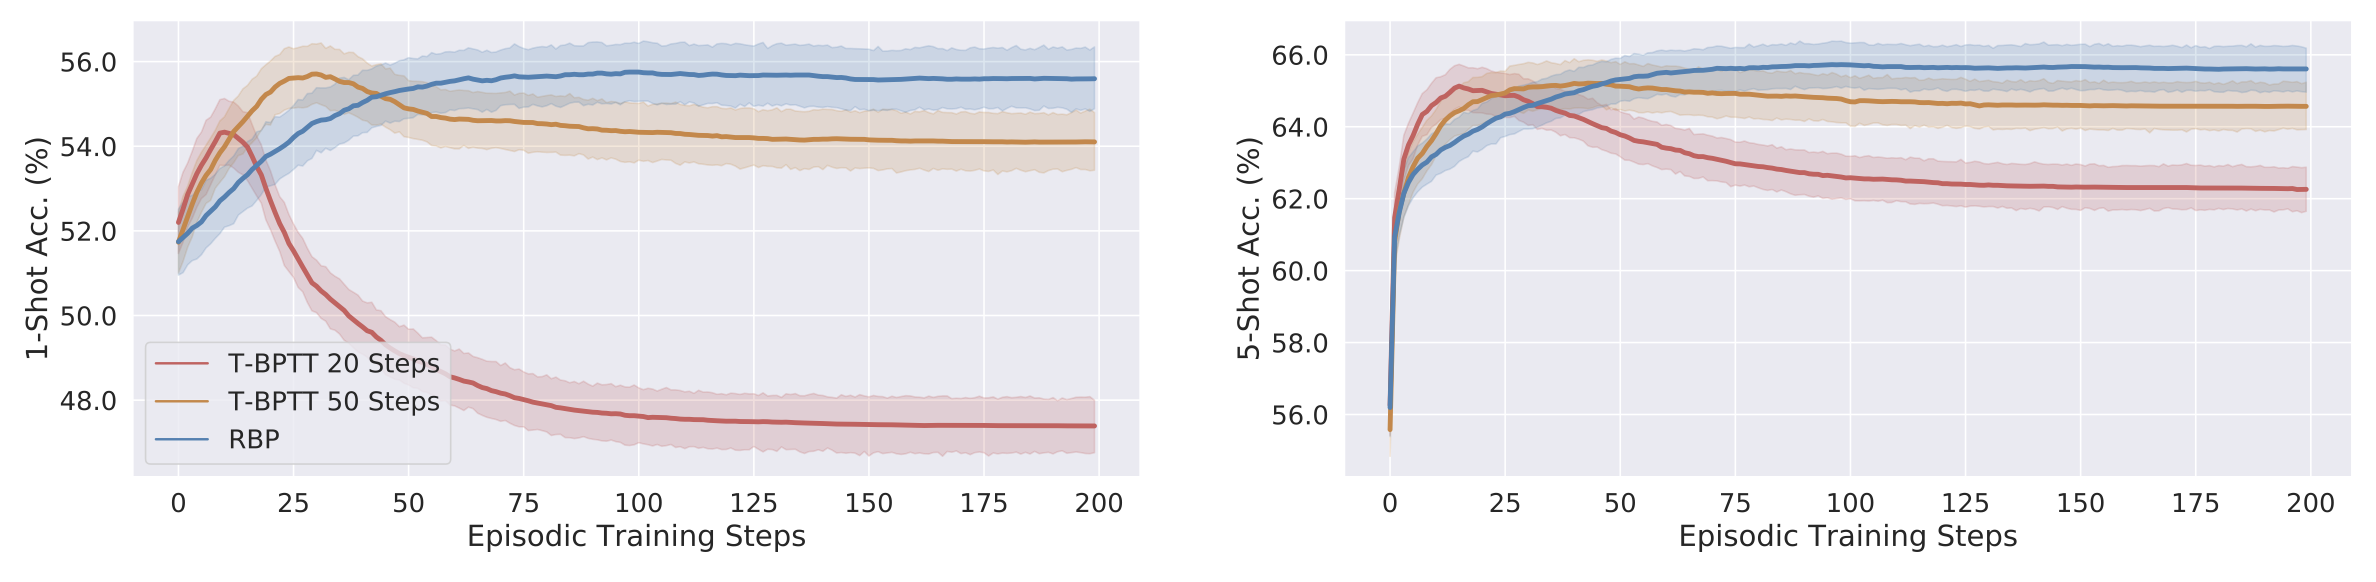
\includegraphics[width=6\textwidth]{figures/bptt.png}
\else
\begin{minipage}[c]{\textwidth}
\centering
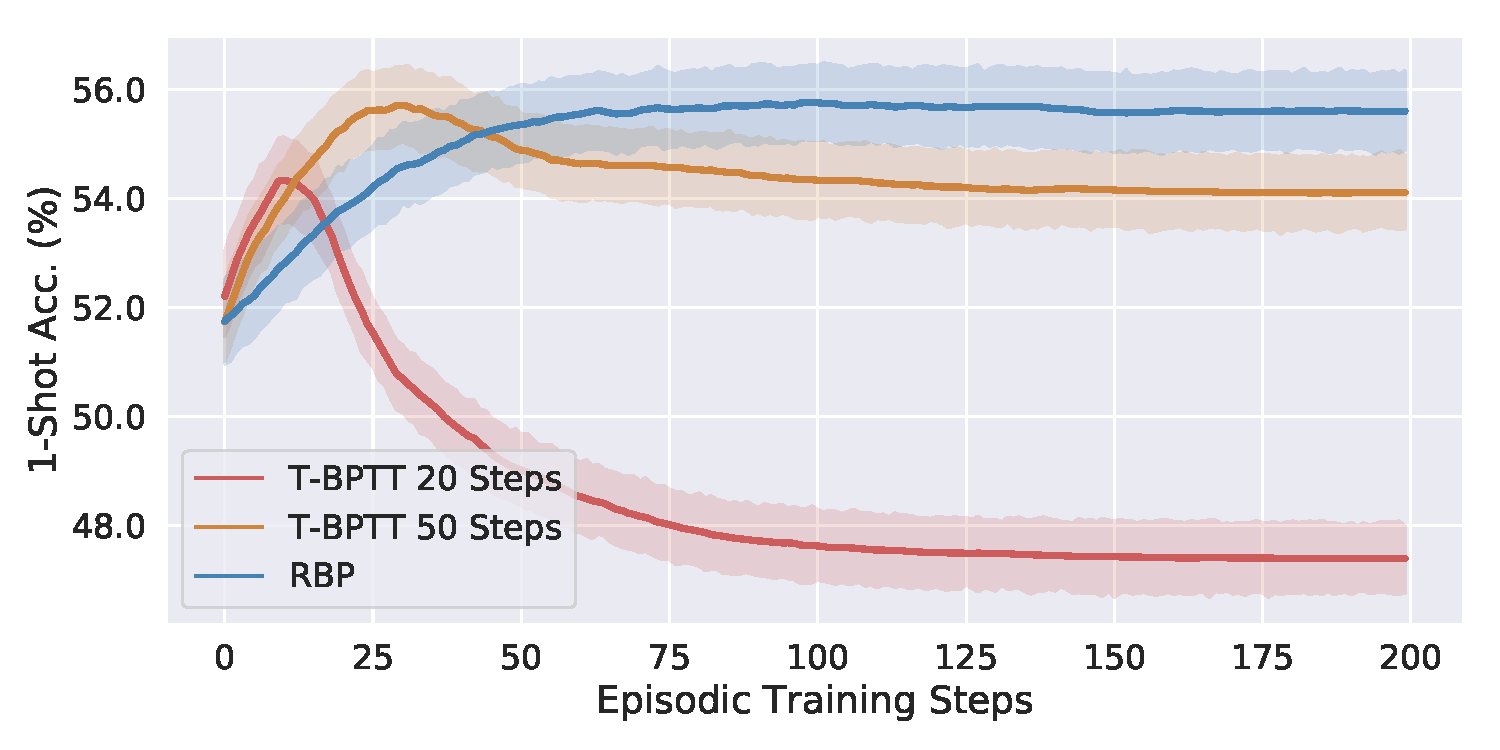
\includegraphics[width=0.49\textwidth,trim={0cm 0cm 0cm 0cm},clip]{figures/example.pdf}
\hfill
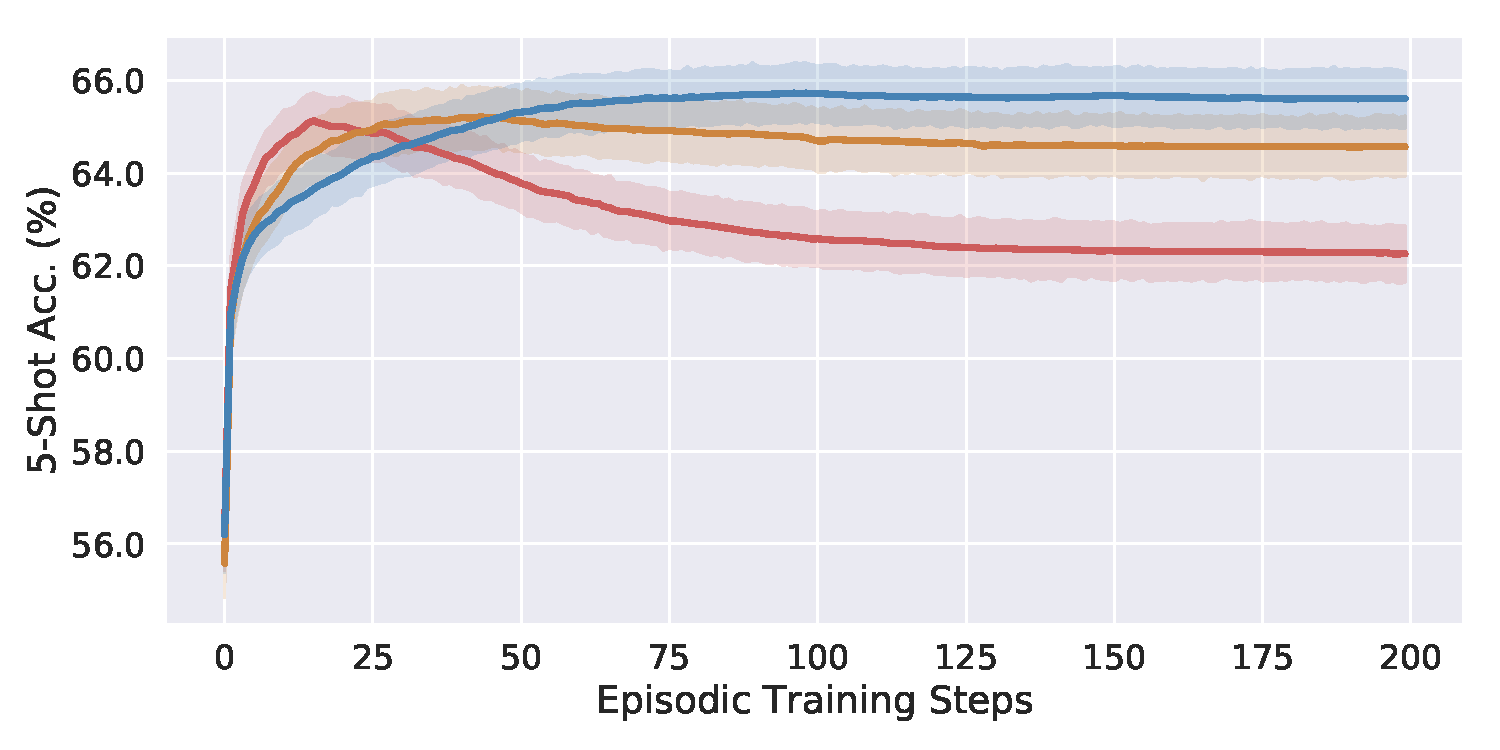
\includegraphics[width=0.49\textwidth,trim={0cm 0cm 0cm 0cm},clip]{figures/example-s5.pdf}
\end{minipage}
\fi
\caption{Learning the proposed model using truncated BPTT vs. RBP. Models
are evaluated with 1-shot (left) and 5-shot (right) 64+5-way episodes,
with various number of gradient descent steps.}
\label{fig:bptt}
\end{figure}
% !TEX root = ../main.tex
\begin{figure}[t]
\vspace{-0.2in}
\centering
\iflatexml
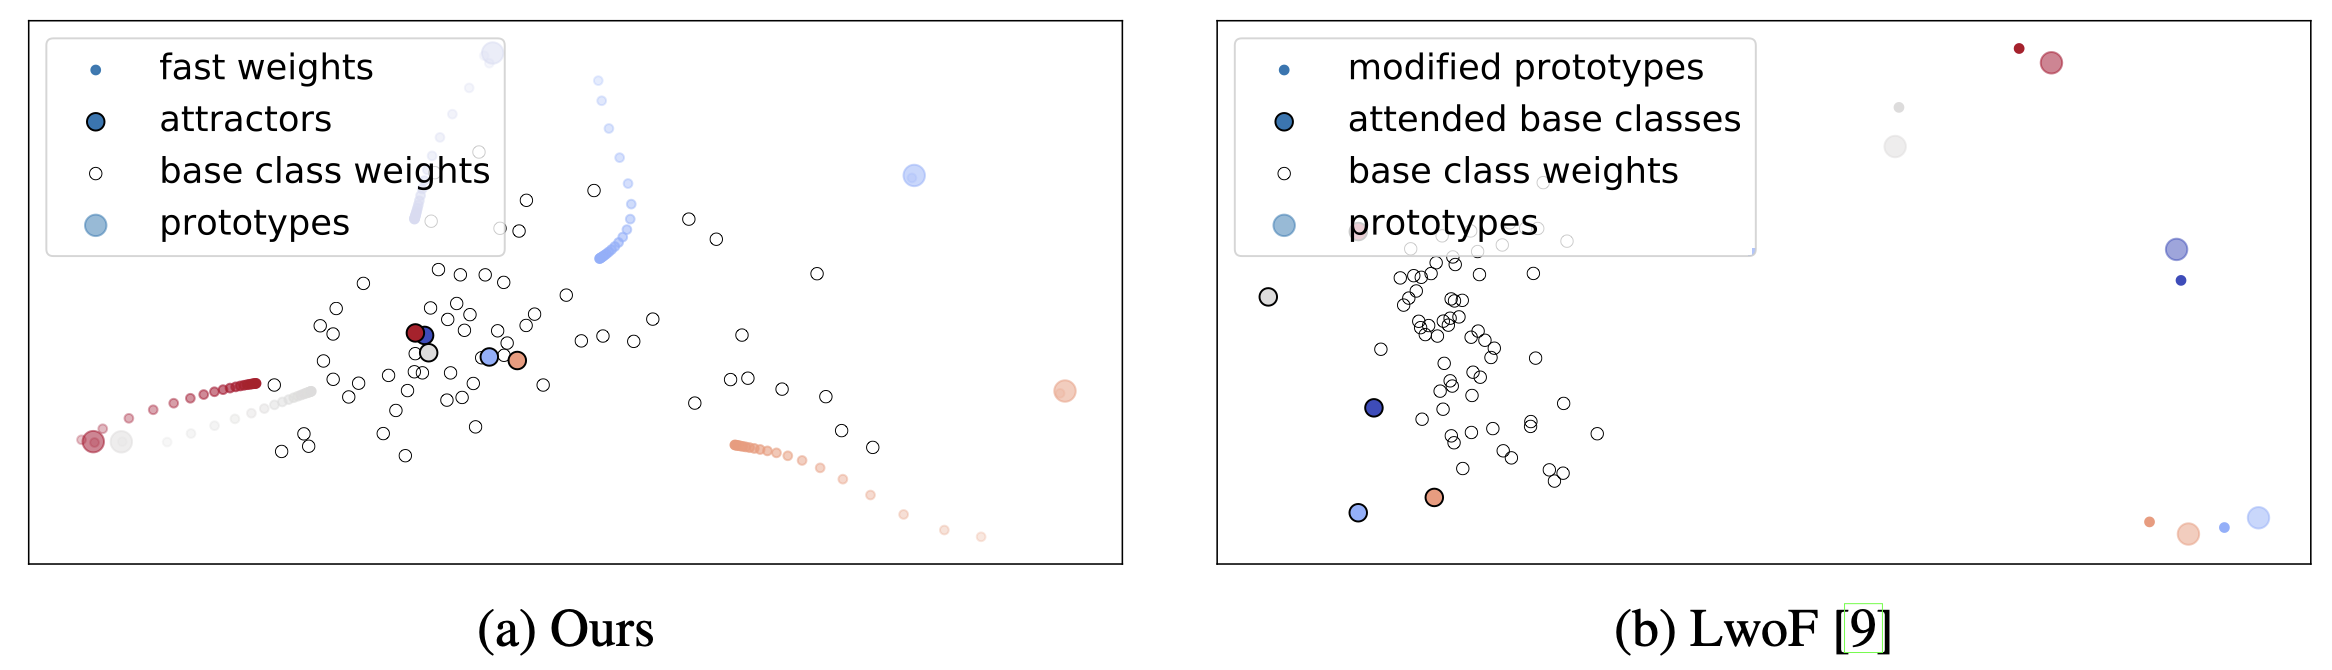
\includegraphics[width=6\textwidth]{figures/attractor_progress.png}
\else
\begin{minipage}[c]{\textwidth}
\centering
\begin{small}
\begin{tabular}{cc}
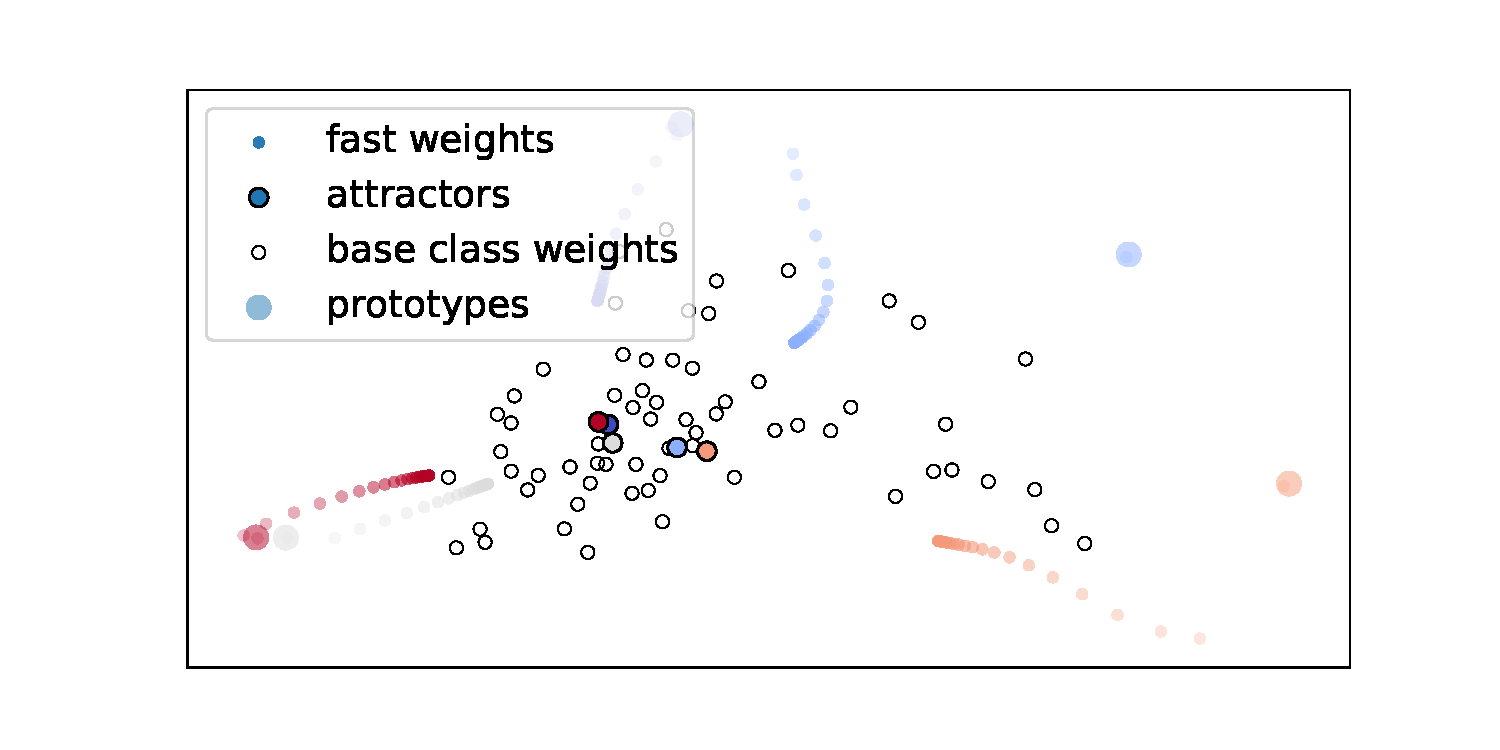
\includegraphics[width=0.47\textwidth,trim={2.8cm 1cm 2.5cm 1cm},clip]{figures/attractor_progress_9.pdf} & 
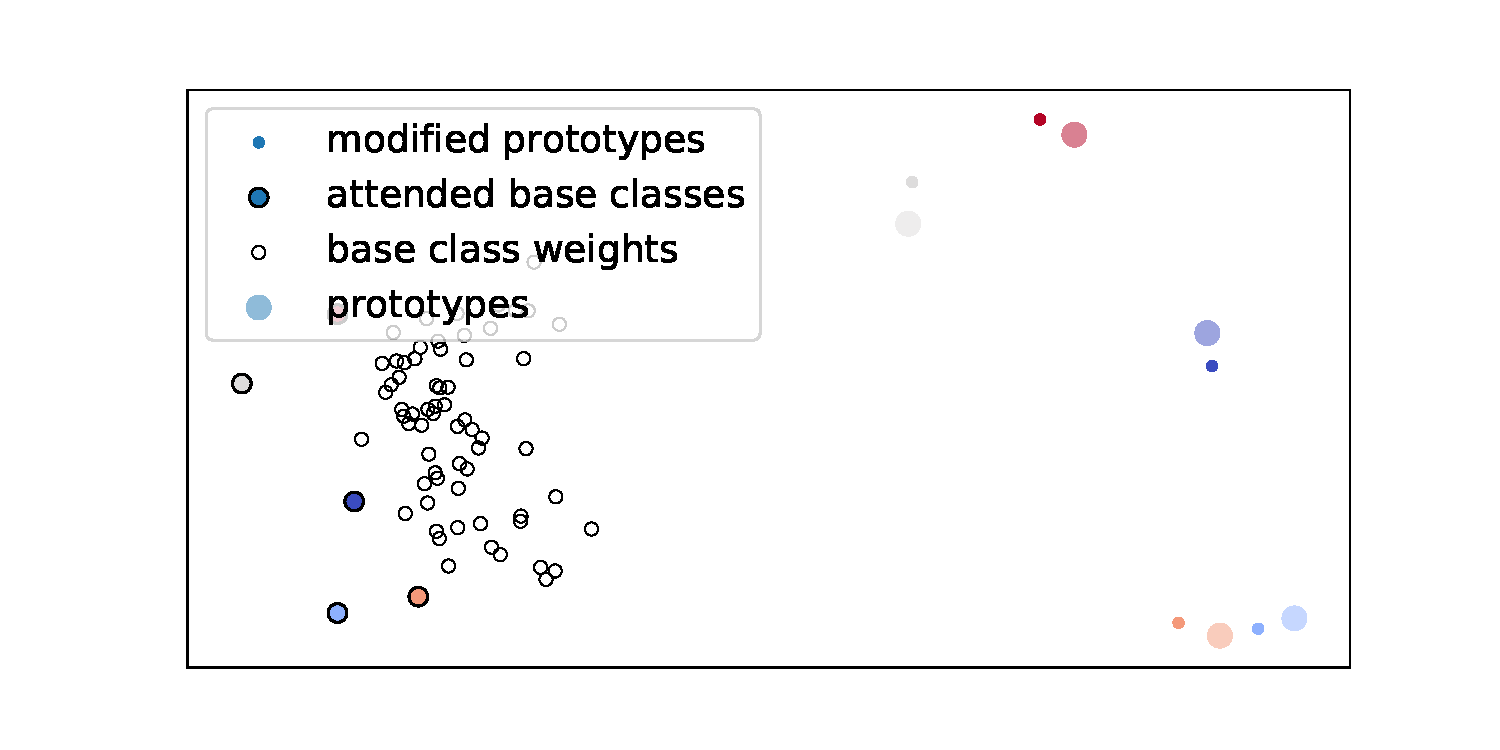
\includegraphics[width=0.47\textwidth,trim={2.8cm 1cm 2.5cm 1cm},clip]{figures/lwof_progress_9.pdf}\\
(a) Ours & (b) LwoF \cite{lwof}
\end{tabular}
\end{small}
\end{minipage}
\fi
\caption{Visualization of a 5-shot 64+5-way episode using PCA. 
\textbf{Left:} Our attractor model learns to
``pull'' prototypes (large colored circles) towards base class weights (white circles). We visualize the trajectories during episodic training; \textbf{Right:} Dynamic few-shot learning without
forgetting \cite{lwof}.}
\label{fig:vizproc}
\vspace{-0.1in}
\end{figure}
% !TEX root = ../main.tex
\iflatexml
\begin{figure}
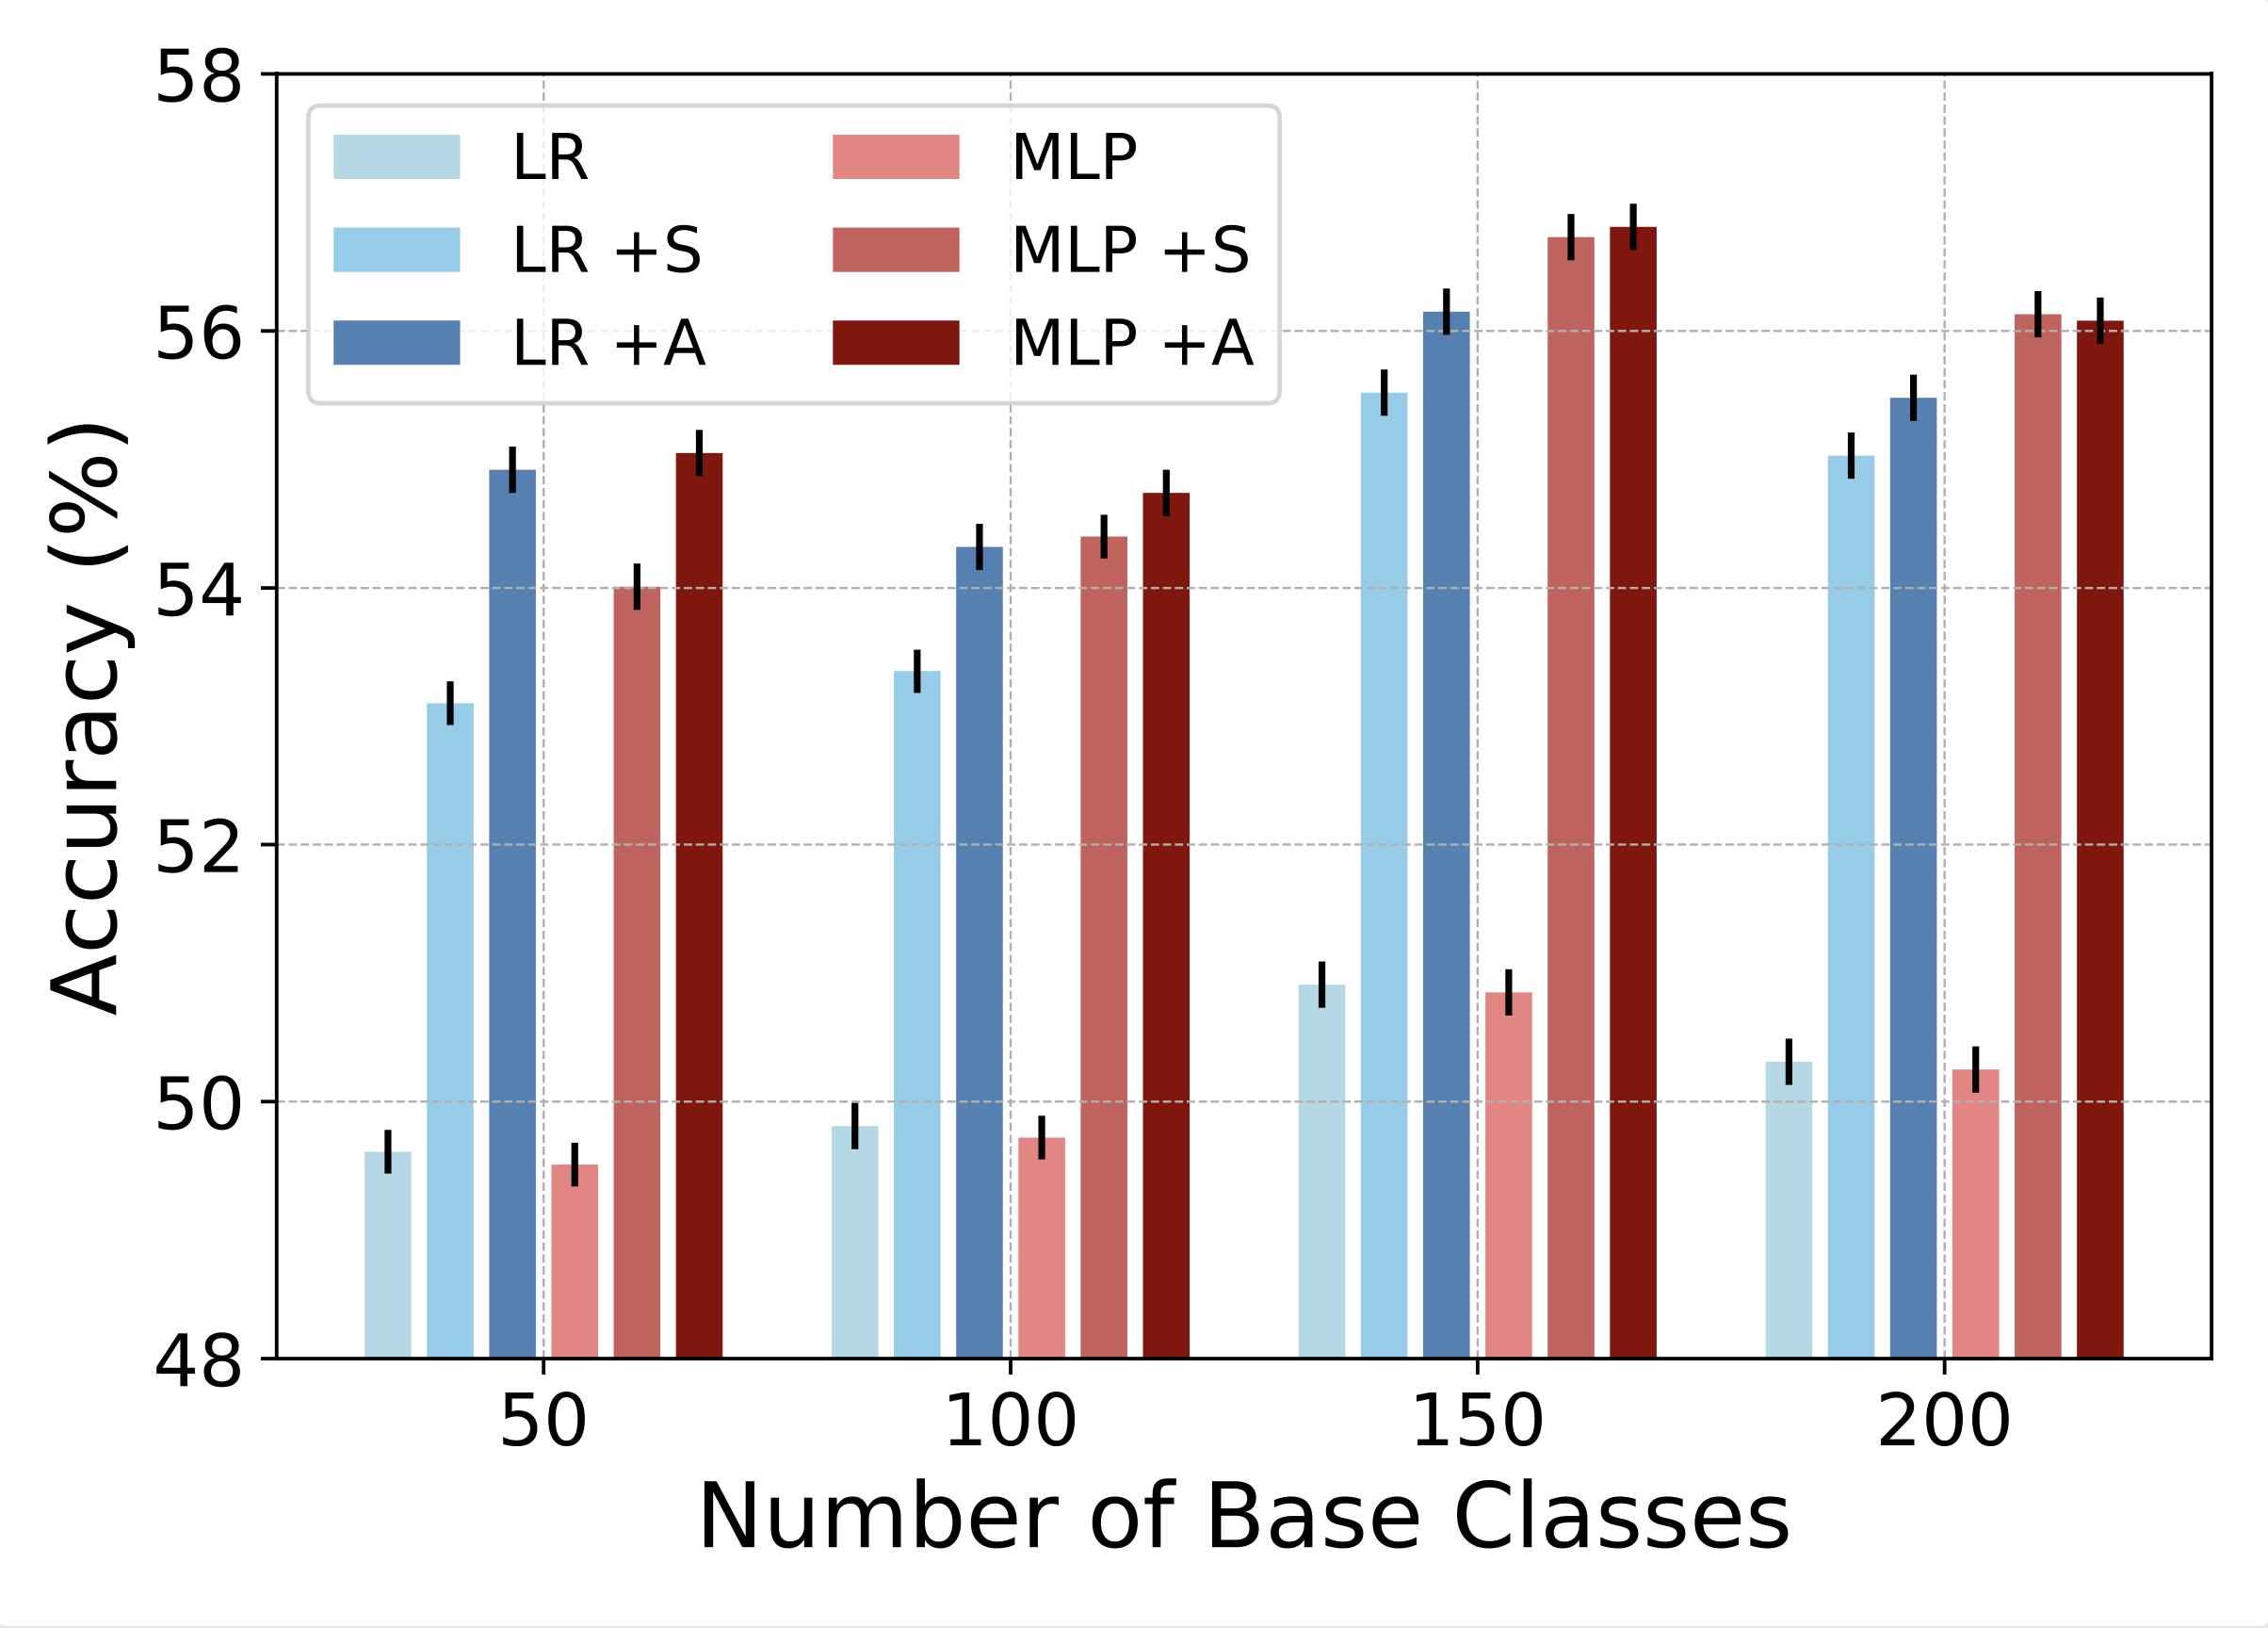
\includegraphics[width=4\textwidth]{figures/snapshot.png}
\caption{Results on \textit{tiered}-ImageNet with \{50, 100, 150, 200\} base classes.
\end{figure}
\else
\begin{wrapfigure}{R}{0.5\textwidth}
\vspace{-0.1in}
\centering
\hfill
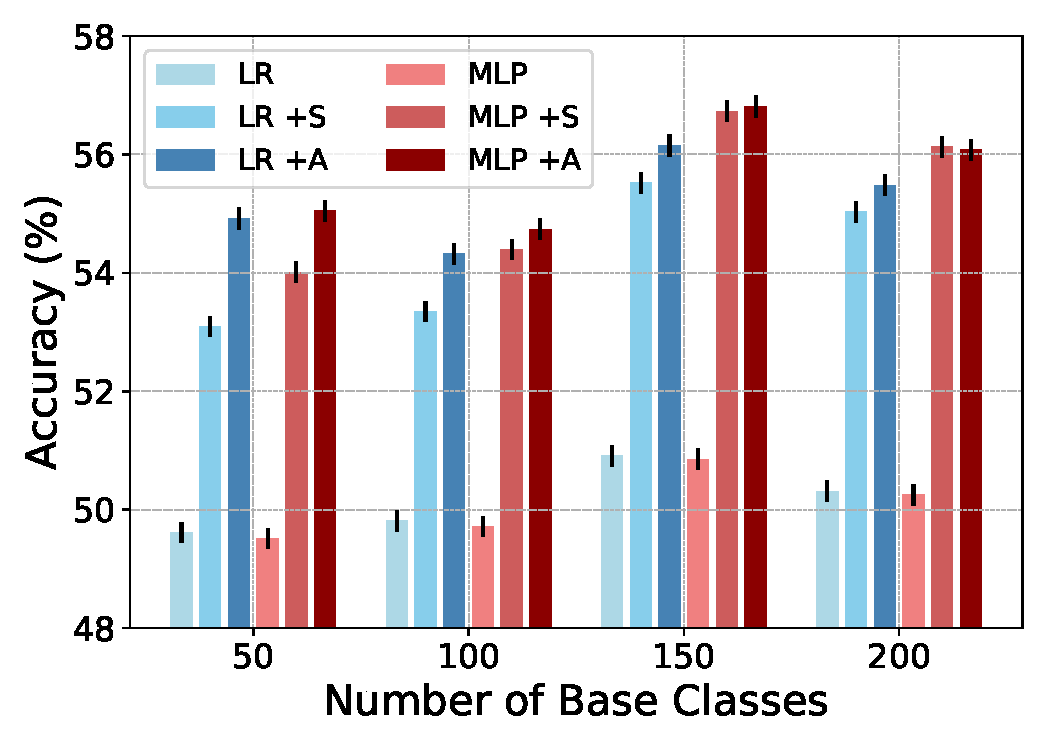
\includegraphics[width=0.5\textwidth,trim={0cm 0cm 0cm 0cm},clip]{figures/snapshot.pdf}
\caption{Results on \textit{tiered}-ImageNet with \{50, 100, 150, 200\} base classes.
}
\label{fig:snapshot}
\vspace{-0.25in}
\end{wrapfigure}
\fi
\paragraph{Comparison to truncated BPTT (T-BPTT)}
An alternative way to learn the regularizer is to unroll the inner optimization for a fixed number
of steps in a differentiable computation graph, and then back-propagate through time. Truncated BPTT
is a popular learning algorithm in many recent meta-learning 
approaches~\citep{gd2,metalstm,maml,mbpa,metareg}. Shown in Figure~\ref{fig:bptt}, the performance of T-BPTT
learned models are comparable to ours; however, when solved to convergence at test time, the
performance of T-BPTT models drops significantly. This is expected as they are only guaranteed to
work well for a certain number of steps, and failed to learn a good regularizer.
While an early-stopped T-BPTT model can do equally well, in practice it is hard to tell when to stop; whereas for the RBP model, doing the full episodic training is very fast since the number of support examples is small. 

\paragraph{Visualization of attractor dynamics} We visualize attractor dynamics in
Figure~\ref{fig:vizproc}. Our learned attractors pulled the fast weights close towards the base
class weights. In comparison, \citet{lwof} only modify the prototypes slightly.

\paragraph{Varying the number of base classes}
While the framework proposed in this paper cannot be directly applied on class-incremental continual
learning, as there is no module for memory consolidation, we can simulate the continual learning
process by varying the number of base classes, to see how the proposed models are affected by
different stages of continual learning. Figure~\ref{fig:snapshot} shows that the learned
regularizers consistently improve over baselines with weight decay only. The overall accuracy
increases from 50 to 150 classes due to better representations on the backbone network, and drops
at 200 classes due to a more challenging classification task.